So far, we have looked at linear models of the form
\begin{align}
	Y_i = \beta_0 + \beta_1x_{1i} + \beta_2x_{2i} + \dots + \beta_px_{pi} + \epsilon_i\notag
\end{align}
In this lecture, we extend this concept:
\begin{itemize}
	\item We look at how we can use different types of predictors to capture a wide range of relationships (e.g. capture non-linear relationship with linear model).
	\item We'll think about how to formulate models, depending on their use.
	\item We'll consider some common pitfalls in use of linear models.
\end{itemize}

\begin{example}
	Consider energy usage in houses, based on their size.
	\begin{center}
		\begin{tikzpicture}[scale=0.9]
			\begin{axis}[
				xmin=0, xmax=3, xlabel=$x$,
				ymin=4, ymax=8, ylabel=$y$,
				title=\textbf{Linear fit},
				axis x line=middle,
				axis y line=middle,
				samples=400
			]
			\addplot[blue, mark=x, only marks] coordinates	{
				(0.00,4.00)
				(0.10,4.42)
				(0.20,4.81)
				(0.30,5.18)
				(0.40,5.51)
				(0.50,5.82)
				(0.60,6.11)
				(0.70,6.37)
				(0.80,6.60)
				(0.90,6.81)
				(1.00,7.00)
				(1.10,7.17)
				(1.20,7.31)
				(1.30,7.43)
				(1.40,7.53)
				(1.50,7.61)
				(1.60,7.68)
				(1.70,7.72)
				(1.80,7.75)
				(1.90,7.75)
				(2.00,7.75)
				(2.10,7.72)
				(2.20,7.68)
				(2.30,7.63)
				(2.40,7.56)
				(2.50,7.48)
				(2.60,7.39)
				(2.70,7.28)
				(2.80,7.16)
				(2.90,7.03)
			};
			\addplot[mark=none] {0.96*x+5.4};
			\end{axis}
		\end{tikzpicture}
		\begin{tikzpicture}[scale=0.9]
		\begin{axis}[
		xmin=0, xmax=3, xlabel=$x$,
		ymin=4, ymax=8, ylabel=$y$,
		title=\textbf{Polynomial fit},
		axis x line=middle,
		axis y line=middle,
		samples=400
		]
		\addplot[blue, mark=x, only marks] coordinates	{
			(0.00,4.00)
			(0.10,4.42)
			(0.20,4.81)
			(0.30,5.18)
			(0.40,5.51)
			(0.50,5.82)
			(0.60,6.11)
			(0.70,6.37)
			(0.80,6.60)
			(0.90,6.81)
			(1.00,7.00)
			(1.10,7.17)
			(1.20,7.31)
			(1.30,7.43)
			(1.40,7.53)
			(1.50,7.61)
			(1.60,7.68)
			(1.70,7.72)
			(1.80,7.75)
			(1.90,7.75)
			(2.00,7.75)
			(2.10,7.72)
			(2.20,7.68)
			(2.30,7.63)
			(2.40,7.56)
			(2.50,7.48)
			(2.60,7.39)
			(2.70,7.28)
			(2.80,7.16)
			(2.90,7.03)
		};
		\addplot[mark=none] {0.1089*x^3-1.453*x^2+4.344*x+4};
		\end{axis}
		\end{tikzpicture}
	\end{center}
\end{example}

A simple linear models might tell us that a predictor is important, but it's no good prediction. Model building is a process that includes:
\begin{itemize}
	\item \textbf{Formulating a model:} model structure, we'll look at different types of predictors today.
	\item \textbf{Model fitting:} last two lectures
	\item \textbf{Model evaluation:} Check model assumptions hold, avoid common pitfalls
\end{itemize}

Before formulating a statistical model, it is good practice to explore the data. Look at scatter plots of predictors against the response and predictors against each other. Can help to develop an intuition for model structure. Look at distributions of response and predictors (e.g. look for outliers, can you capture the distribution with your model?) Think about what the model will be used for (e.g. prediction, or simply to find relevant explanatory variables).

\subsection{Types of predictors}

\subsubsection{qualitative vs quantitative}

So far, we have looked at \begriff{quantitative predictors} (numerical variables), e.g. temperature, energy usage, waiting time before computer processes data, ... But we can have \begriff{qualitative predictors} as well (categorical variables), e.g. type of engine, type fuel used, type of processor used, ... These are included in models using \begriff{dummy variables}.

\begin{example}
	Consider the performance $Y_i$ of diesel engines for three different fuel types A, B and C. We use the model $Y_i = \beta_0 + \beta_1x_{1i} + \beta_2x_{2i} + \epsilon_i$, where $x_{1i}$ and $x_{2i}$ are dummy variables such that
	\begin{align}
		x_{1i} &= \begin{cases}
		1 & \text{if fuel B is used} \\ 0 & \text{if not}
		\end{cases} \notag \\
		x_{2i} &= \begin{cases}
		1 & \text{if fuel C is used} \\ 0 & \text{if not}
		\end{cases} \notag 
	\end{align}
	The performance for fuel type A is captured in $\beta_0$.
\end{example}

Qualitative and quantitative predictors can be combined in models.

\begin{example}
	Consider fuel efficiency of car models from the 1950s (\textcolor{blue}{type 1}) and from the 1960s (\textcolor{red}{type 2}), depending on their weight. For car models $i=1,...,n$, we might consider the model $Y_i = \beta_0 + \beta_1x_i + \beta_2w_i + \epsilon_i$, where $Y_i$ is the efficiency in miles per gallon (MPG), $x_i$ is a dummy variable for the car type and $w_i$ is the weight of a car model. We might find:
	\begin{center}
	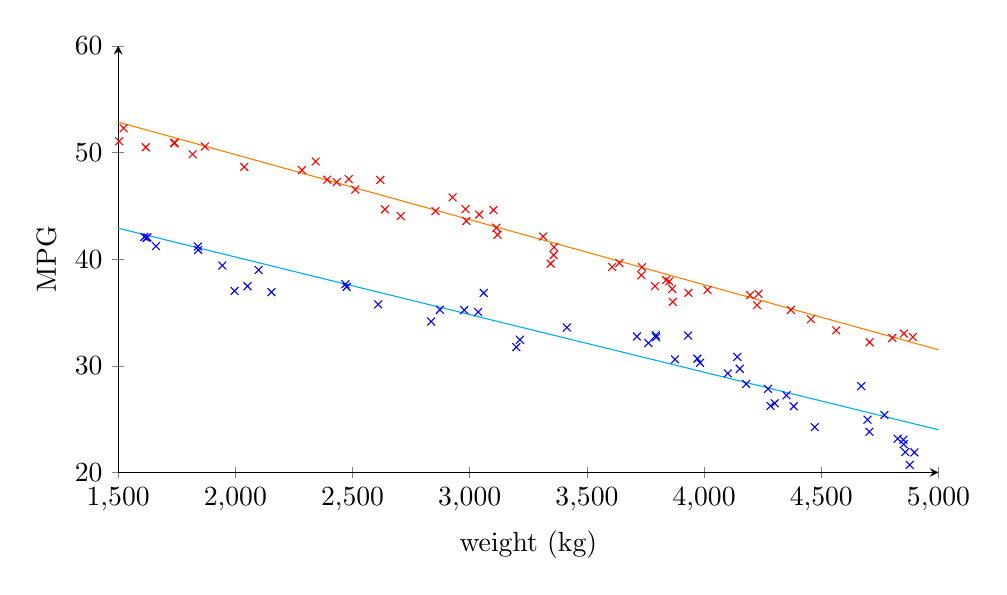
\begin{tikzpicture}
		\begin{axis}[
		xmin=1500, xmax=5000, xlabel=weight (kg),
		ymin=20, ymax=60, ylabel=MPG,
		axis x line=bottom,
		axis y line=left,
		samples = 400,
		height=7cm,
		width=12cm,
		domain=1500:5000
		]
		\addplot[blue, mark=x, only marks] coordinates {
			(1611.41,42.08)
			(1620.56,42.00)
			(1624.99,42.04)
			(1661.60,41.22)
			(1839.96,41.19)
			(1841.39,40.86)
			(1944.45,39.40)
			(1996.60,37.02)
			(2051.65,37.46)
			(2099.15,38.98)
			(2154.05,36.90)
			(2469.23,37.65)
			(2474.74,37.40)
			(2609.85,35.76)
			(2835.45,34.15)
			(2872.79,35.25)
			(2976.16,35.22)
			(3035.61,35.04)
			(3059.55,36.83)
			(3198.81,31.75)
			(3214.18,32.44)
			(3414.09,33.59)
			(3713.26,32.75)
			(3762.10,32.13)
			(3794.17,32.87)
			(3795.09,32.68)
			(3875.57,30.60)
			(3931.90,32.84)
			(3971.16,30.67)
			(3982.78,30.28)
			(4100.96,29.29)
			(4141.40,30.83)
			(4152.09,29.72)
			(4179.31,28.30)
			(4272.73,27.84)
			(4283.20,26.24)
			(4300.98,26.48)
			(4351.53,27.23)
			(4382.10,26.20)
			(4471.95,24.25)
			(4670.27,28.10)
			(4696.82,24.95)
			(4705.07,23.82)
			(4768.98,25.39)
			(4825.78,23.16)
			(4850.08,23.07)
			(4851.27,22.65)
			(4858.22,21.91)
			(4877.11,20.71)
			(4897.07,21.88)
		};
		\addplot[red,mark=x,only marks] coordinates {
			(1504.03,51.05)
			(1523.50,52.27)
			(1617.61,50.49)
			(1737.97,50.88)
			(1740.82,50.90)
			(1817.88,49.83)
			(1869.70,50.56)
			(2037.80,48.64)
			(2284.14,48.35)
			(2342.47,49.15)
			(2391.77,47.45)
			(2432.65,47.22)
			(2483.52,47.50)
			(2511.73,46.52)
			(2618.60,47.43)
			(2638.01,44.67)
			(2705.62,44.04)
			(2853.70,44.50)
			(2926.67,45.79)
			(2982.09,44.69)
			(2985.22,43.58)
			(3040.30,44.18)
			(3100.99,44.60)
			(3113.21,42.94)
			(3118.57,42.29)
			(3313.18,42.12)
			(3345.00,39.58)
			(3358.02,40.38)
			(3359.67,41.13)
			(3607.60,39.26)
			(3638.36,39.63)
			(3731.98,38.49)
			(3734.86,39.25)
			(3790.56,37.47)
			(3837.41,38.04)
			(3851.33,37.91)
			(3863.66,37.21)
			(3866.43,35.99)
			(3932.99,36.84)
			(4014.26,37.12)
			(4195.56,36.63)
			(4225.81,35.69)
			(4231.82,36.74)
			(4369.93,35.24)
			(4455.37,34.36)
			(4563.80,33.32)
			(4705.97,32.20)
			(4802.68,32.61)
			(4851.93,33.02)
			(4890.27,32.70)
		};
		\addplot[cyan,mark=none] {-0.0054*x+51};
		\addplot[orange,mark=none] {-0.0061*x+62};
		\end{axis}
	\end{tikzpicture}
\end{center}
\end{example}

\subsubsection{interaction terms}

So far, we have assumed that the effects of all explanatory variables are additive, e.g. as is $Y_i = \beta_0 + \beta_1x_{1i} + \beta_2x_{2i} + \epsilon_i$. What if the relationship between $Y_i$ and $x_{1i}$ depends on the value of $x_{2i}$? 

Then we need to consider \begriff{interaction terms} in our model, e.g. $Y_i = \beta_0 + \beta_1x_{1i} + \beta_2x_{2i} + \beta_3x_{1i}x_{2i} + \epsilon_i$. Interpretation of model parameters:
\begin{itemize}
	\item $(\beta_1 + \beta_3x_2)$ represents the change in $Y$ for every unit increase in $x_1$, holding $x_2$ fixed.
	\item $(\beta_2 + \beta_3x_1)$ represents the change in $Y$ for every unit increase in $x_2$, holding $x_1$ fixed.
	\item In model checking: if interaction term is important, then the interacting explanatory variable must be important and t-tests on them are meaningless.
\end{itemize}

This is still a linear model - the effects captured by parameters are additive.

\begin{example}
	Fuel efficiency $Y_i$ of car models from \textcolor{blue}{1970}, \textcolor{red}{'76} and \textcolor{green}{'82} depending on their weight $w_i$. Consider interaction between year built and weight.
	\begin{align}
		Y_i = \beta_0 + \beta_1x_{1i} + \beta_2x_{2i} + \beta_3w_i + \beta_4x_{1i}w_i + \beta_5x_{2i}w_i + \epsilon_i\notag
	\end{align}
	This model has main effects for year and weight and interaction terms. Model fitting:
	\begin{center}
	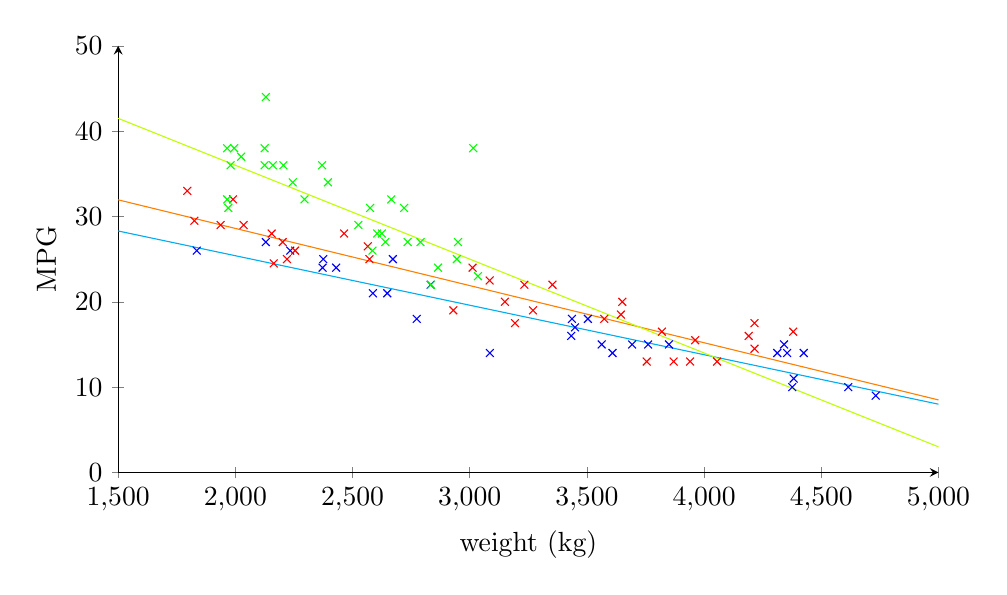
\begin{tikzpicture}
		\begin{axis}[
		xmin=1500, xmax=5000, xlabel=weight (kg),
		ymin=0, ymax=50, ylabel=MPG,
		axis x line=bottom,
		axis y line=left,
		samples = 400,
		height=7cm,
		width=12cm,
		domain=1500:5000
		]
		\addplot[blue, mark=x, only marks] coordinates {
			(3504.00,18.00)
			(3693.00,15.00)
			(3436.00,18.00)
			(3433.00,16.00)
			(3449.00,17.00)
			(4341.00,15.00)
			(4354.00,14.00)
			(4312.00,14.00)
			(4425.00,14.00)
			(3850.00,15.00)
			(3563.00,15.00)
			(3609.00,14.00)
			(3761.00,15.00)
			(3086.00,14.00)
			(2372.00,24.00)
			(2833.00,22.00)
			(2774.00,18.00)
			(2587.00,21.00)
			(2130.00,27.00)
			(1835.00,26.00)
			(2672.00,25.00)
			(2430.00,24.00)
			(2375.00,25.00)
			(2234.00,26.00)
			(2648.00,21.00)
			(4615.00,10.00)
			(4376.00,10.00)
			(4382.00,11.00)
			(4732.00,9.00)
		};
		\addplot[red,mark=x,only marks] coordinates {
			(2464.00,28.00)
			(2220.00,25.00)
			(2572.00,25.00)
			(2255.00,26.00)
			(2202.00,27.00)
			(4215.00,17.50)
			(4190.00,16.00)
			(3962.00,15.50)
			(4215.00,14.50)
			(3233.00,22.00)
			(3353.00,22.00)
			(3012.00,24.00)
			(3085.00,22.50)
			(2035.00,29.00)
			(2164.00,24.50)
			(1937.00,29.00)
			(1795.00,33.00)
			(3651.00,20.00)
			(3574.00,18.00)
			(3645.00,18.50)
			(3193.00,17.50)
			(1825.00,29.50)
			(1990.00,32.00)
			(2155.00,28.00)
			(2565.00,26.50)
			(3150.00,20.00)
			(3940.00,13.00)
			(3270.00,19.00)
			(2930.00,19.00)
			(3820.00,16.50)
			(4380.00,16.50)
			(4055.00,13.00)
			(3870.00,13.00)
			(3755.00,13.00)
		};
		\addplot[green,mark=x,only marks] coordinates {
			(2605.00,28.00)
			(2640.00,27.00)
			(2395.00,34.00)
			(2575.00,31.00)
			(2525.00,29.00)
			(2735.00,27.00)
			(2865.00,24.00)
			(3035.00,23.00)
			(1980.00,36.00)
			(2025.00,37.00)
			(1970.00,31.00)
			(2125.00,38.00)
			(2125.00,36.00)
			(2160.00,36.00)
			(2205.00,36.00)
			(2245.00,34.00)
			(1965.00,38.00)
			(1965.00,32.00)
			(1995.00,38.00)
			(2945.00,25.00)
			(3015.00,38.00)
			(2585.00,26.00)
			(2835.00,22.00)
			(2665.00,32.00)
			(2370.00,36.00)
			(2950.00,27.00)
			(2790.00,27.00)
			(2130.00,44.00)
			(2295.00,32.00)
			(2625.00,28.00)
			(2720.00,31.00)
		};
		\addplot[cyan,mark=none] {-0.0058*x+37};
		\addplot[orange,mark=none] {-0.0067*x+42};
		\addplot[lime,mark=none] {-0.011*x+58};
		\end{axis}
	\end{tikzpicture}
\end{center}
	To test if interactions are important, could use the Likelihood-ratio test ($H_0$: $\beta_4=\beta_5=0$).
\end{example}

\subsubsection{polynomials of predictors}

How to deal with non-linear relationships between variables?

Can account for this in models using polynomials of predictors, e.g. $Y_i = \beta_0 + \beta_1x_{1i} + \beta_2x_{1i}^2 + \epsilon_i$, where $\beta_0$ is the intercept, $\beta_1$ is a shift parameter and $\beta_2$ is the rate and direction of curvature. Higher-order polynomials are also possible.

This is still a linear model - the effects captured by parameters are additive.

\begin{example}
	Consider data on energy usage in houses depending on their size and second-order model $Y_i = \beta_0 + \beta_1x_{1i} + \beta_2x_{1i}^2 + \epsilon_i$.
	\begin{center}
		\begin{tikzpicture}
		\begin{axis}[
		xmin=0, xmax=3, xlabel=$x$,
		ymin=4, ymax=8, ylabel=$y$,
		axis x line=middle,
		axis y line=middle,
		samples=400
		]
		\addplot[blue, mark=x, only marks] coordinates	{
			(0.00,4.00)
			(0.10,4.42)
			(0.20,4.81)
			(0.30,5.18)
			(0.40,5.51)
			(0.50,5.82)
			(0.60,6.11)
			(0.70,6.37)
			(0.80,6.60)
			(0.90,6.81)
			(1.00,7.00)
			(1.10,7.17)
			(1.20,7.31)
			(1.30,7.43)
			(1.40,7.53)
			(1.50,7.61)
			(1.60,7.68)
			(1.70,7.72)
			(1.80,7.75)
			(1.90,7.75)
			(2.00,7.75)
			(2.10,7.72)
			(2.20,7.68)
			(2.30,7.63)
			(2.40,7.56)
			(2.50,7.48)
			(2.60,7.39)
			(2.70,7.28)
			(2.80,7.16)
			(2.90,7.03)
		};
		\addplot[mark=none] {0.1089*x^3-1.453*x^2+4.344*x+4};
		\end{axis}
		\end{tikzpicture}
	\end{center}
\end{example}

Interpreting model parameters:
\begin{itemize}
	\item $\beta_0$ can only be interpreted directly if range of data includes $x=0$.
	\item $\beta_1$ no longer represents a slope and can't be interpreted in isolation.
	\item The sign of $\beta_2$ indicates the direction of the curvature (concave upward or downward).
\end{itemize}

\textbf{Warning:} polynomials of predictors lead to correlations between predictors by design.

\subsubsection{data transformations}

\begriff{Data transformations} can help to address problems in model fit (e.g. when relationship is not linear, but residuals are normally distributed). There are many data transformations and there are two examples below, but in general I'd recommend to be cautious about this.
\begin{itemize}
	\item \begriff{Log-transform predictors}, response or both
	\item \begriff{Code predictors}, so that their range is similar. E.g. for temperature $T$, code this as $x=\frac{T-100}{50}$. Can reduce computational rounding errors in model fit and can help to address problems with multicollinearity in polynomial regression models.
\end{itemize}

\textbf{Warning:} Data transformations do make residuals more normal and statistical tests performed on transformed data are not necessarily relevant for the original data.\footnote{\person{Feng} et al. (2014) \textit{Shanghai Arch Psychiatry}. 26: 105-109}

\subsection{Pitfalls}

Often there is not one correct way to build a model, especially for large data sets with many predictors.

\begin{proposition}[\person{George Box}, 1919-2013]
	Essentially, all models are wrong, but some are useful.
\end{proposition} 

Whether a model is useful or not often depends on how it is used. Things to consider are: prediction or data analysis, exploratory or for decision-making. There are many wrong ways of doing things. Common pitfalls are listed in the following.
\begin{itemize}
	\item \textbf{Multicollinearity} arises when predictors are correlated. This can be data-based or structural when new predictors are created from existing ones (e.g. in polynomial regression). This causes problems: parameter estimates can't be interpreted sensibly and statistical tests on them are meaningless. However, prediction from models within the range covered by the data is not affected by multicollinearity.
	\item \textbf{Model assumptions are violated.} See previous lectures for model assumptions (e.g. normality and independence of errors).
	\item \textbf{Extrapolation beyond the scope of the model.} Trends identified in data by a model do not necessarily hold beyond the range of the data\footnote{\url{https://xkcd.com/605/}}.
	\item \textbf{Excluding important predictors.} Can lead to models that contain misleading associations between variables. Avoid by data exploration and considering background information on data.
	\item \textbf{Parameter interpretation.} A common misconception is that parameter estimates always measure the effect of a predictor on the response independent from other predictors (e.g. not the case in models with interactions). Another misinterpretation is that significant p-values for a parameter indicate a cause-and-effect relationship. Unless we control for all other effects, they do not.
	\item \textbf{Overfitting.} Recall \person{Occam}'s Razor (\cref{occams_razor}). An extreme case of overfitting is to use as many model parameters as there are data points. In less extreme cases, including too many predictors makes interpretation difficult.
	\item \textbf{Power and sample size.} Small data sets can lead to poorly fitted models with large standard errors for parameter estimates. The more data, the better. General guidelines, such as number of data points per predictor, are not possible, as they depend on the context (e.g. effect size, variability in the data).
\end{itemize}